\documentclass[12pt,oneside,a4]{article}
\usepackage{float}
\usepackage[utf8]{inputenc}
\usepackage[a4paper,width=160mm,top=25mm,bottom=25mm]{geometry}
% \usepackage[lining,tabular]{fbb} % so math uses tabular lining figures
\usepackage{graphicx}
\usepackage{enumitem}
\usepackage{pdflscape}
\usepackage[table]{xcolor}
\usepackage{booktabs}
\usepackage{chngpage}
\usepackage{scrextend}

\usepackage[hidelinks]{hyperref}
\graphicspath{{figures/}} %Setting the graphicspath
\renewcommand\abstractname{\large Introduction}

\renewcommand{\familydefault}{\sfdefault}
\let\tempone\itemize
\let\temptwo\enditemize
\renewenvironment{itemize}{\tempone\addtolength{\itemsep}{-0.5\baselineskip}}{\temptwo}

\newcommand{\linkdeploy}{https://pie2021-testapp-v17.herokuapp.com/}


\title{Flight Assistant -- Quick Start Guide\\ \small{v. 2022-02}}
\author{Fiona \MakeUppercase{Benedito}, 
		Dinh-Viet-Toan  \MakeUppercase{Le}, 
		Claire \MakeUppercase{Raulin}, 
		Maxime \MakeUppercase{Sabbah}}
\date{}

\begin{document}

\maketitle
\vfill
\begin{center}
    \fbox{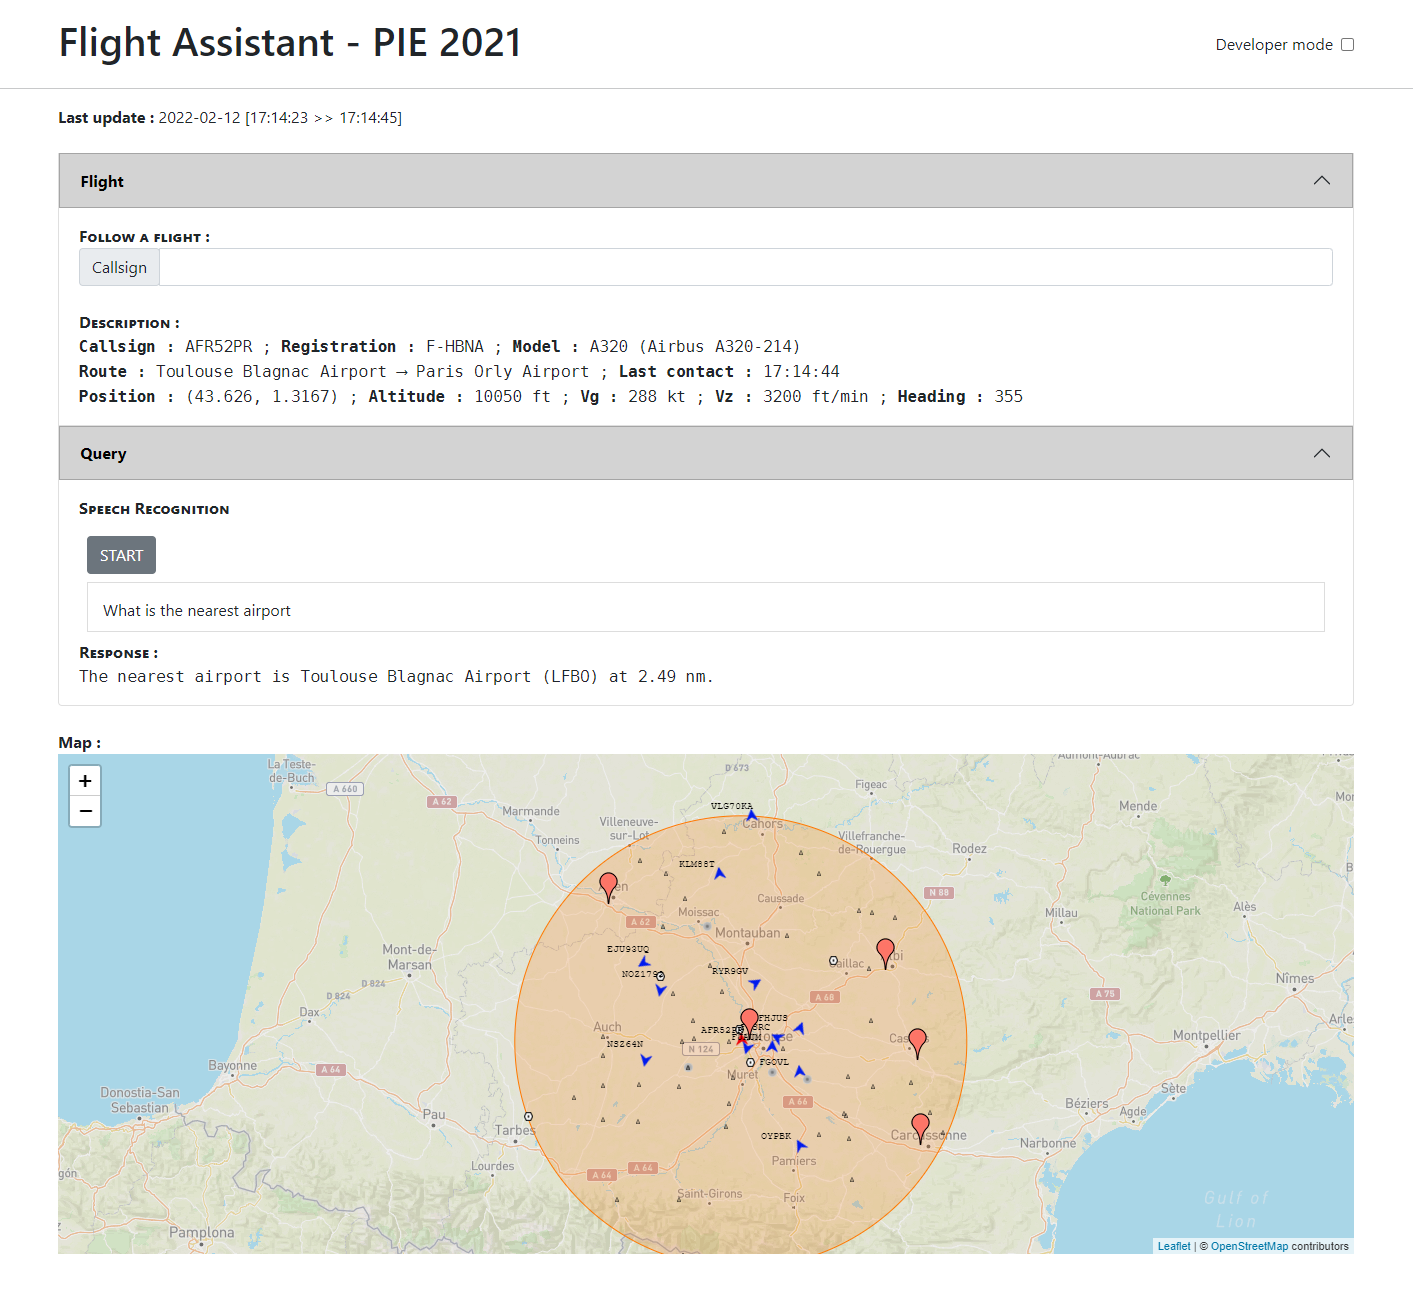
\includegraphics[width=.98\linewidth]{app.png}}
\end{center}
\vfill
\begin{abstract}
Blabla
Dire qu'on se met à la place d'un avion

The app is available here:
\begin{center}
    \vspace{-.5em}
    \url{\linkdeploy}
    \vspace{-.5em}
\end{center}
\end{abstract}

\clearpage
\tableofcontents

\clearpage

% ------------------------------------------------------------------------------

\section{Quick start}

This section will guide you to select a flight, and give instructions on asking queries.

\subsection{Required tools}
\begin{itemize}
    \item \textbf{Chrome} web browser is needed
    \item Microphone
\end{itemize}

\subsection{App launch}
\begin{itemize}
    \item Go to the following webpage : 
    \begin{center}
        \vspace{-.4em}
        \url{\linkdeploy}
    \end{center}
    \item Allow access to the microphone
\end{itemize}

\subsection{Flight following}

\begin{itemize}
    \item Select a flight to follow it. The easiest way is to click on one of the blue cursors representing the flights on the map (Figure~\ref{fig:select_flight}). 
    Else, you can search a flight by its callsign in the ``Follow a flight'' field (Figure~\ref{fig:search_flight})
    \begin{figure}[h!]
        \centering
        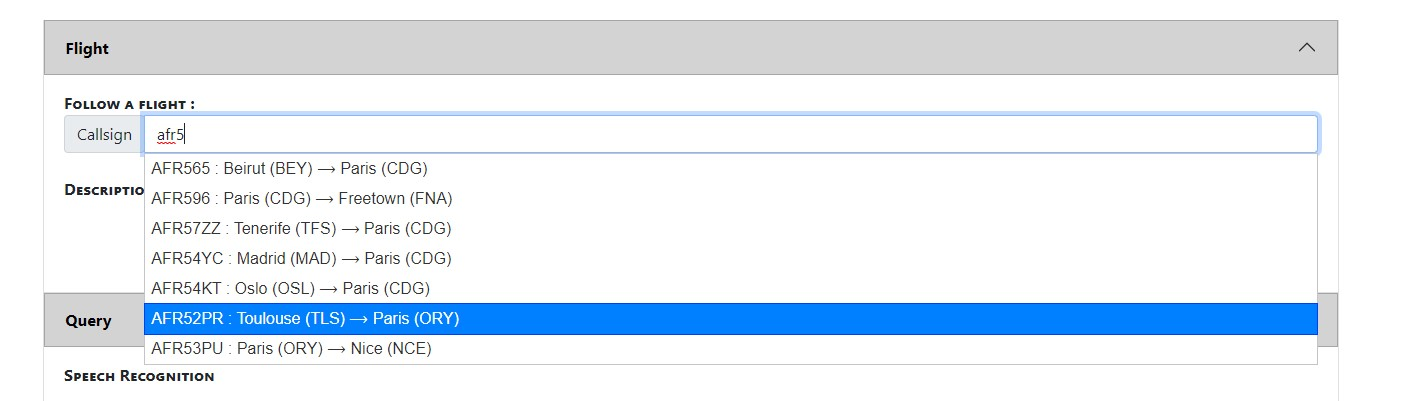
\includegraphics[width=.98\linewidth]{search_flight.jpg}
        \caption{Flight search by callsign}
        \label{fig:search_flight}
    \end{figure}
    \item On the map you may see that the orange zone in the map is centered on the selected flight
    \item The ``START'' button in the Speech Recognition section is also activated.
\end{itemize}

\begin{figure}[h!]
    \centering
    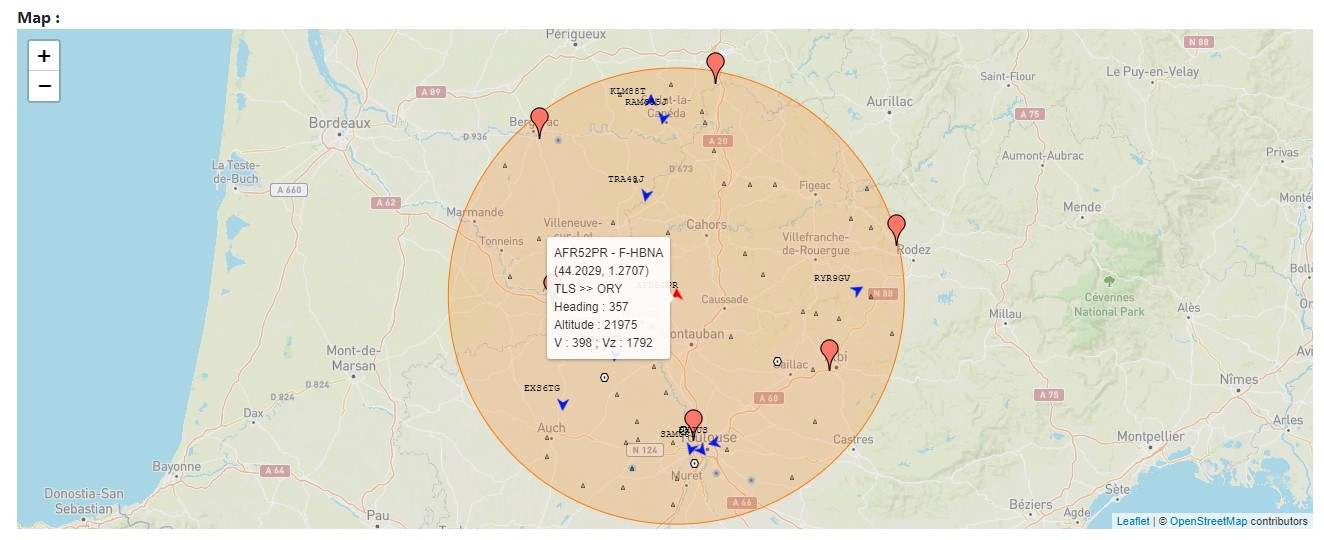
\includegraphics[width=.98\linewidth]{select_flight.jpg}
    \caption{Map after selection of a flight}
    \label{fig:select_flight}
\end{figure}


\subsection{Queries}
Once a flight is selected, you can ask queries to the flight assistant using the push-to-talk button, set to the 'A' key of the keyboard. Queries can be asked either in natural language with plain sentences, or with sequence of specific words.

\begin{itemize}
    \item Push the push-to-talk button ('A' key) and maintain it.
    \item Ask your question. A transcript is also displayed in real-time.
    \item Release the push-to-talk button to send your query.
\end{itemize}

The exhaustive list of implemented queries with a list of possible questions are available at the \hyperref[sec:available-queries]{``Available queries''} section of this document.

% ------------------------------------------------------------------------------
\section{Overview of the user interface}
\begin{figure}[h!]
    \centering
    \includegraphics{example-image-a}
    \caption{User interface}
    \label{fig:user_interface}
\end{figure}


% ------------------------------------------------------------------------------
\section{Queries}
\subsection{Static queries}
Can be [arrival], [departure], [the nearest airport]

\subsection{Dynamic queries}

\subsection{Checklists}

\textit{
Checklists queries have not been implemented depending on the model of the airplane selected. 
These queries are only for test purposes.
}




% ------------------------------------------------------------------------------
\newpage
\begin{landscape}
\thispagestyle{empty}
\section*{Available queries}
\label{sec:available-queries}
\addcontentsline{toc}{section}{Available queries}
\renewcommand{\arraystretch}{1.5}

\begin{table}[!h]

        \centering
        \footnotesize
\begin{tabular}{|p{0.2\paperwidth}|p{0.5\paperwidth}|p{0.4\paperwidth}|}
\hline
\rowcolor{gray} \textbf{Intent} & \textbf{Description} & \textbf{Examples} \\
\hline 

\rowcolor{lightgray} \multicolumn{3}{|l|}{Static queries (that will not change during the flight)} \\ \hline 
Departure / Arrival airport  & Returns the name and the ICAO of the departure / arrival airport & ``What is the arrival airport ?''  \\ 
\hline 
Runways at an airport  & Returns the list of runways at the an airport & ``What are the runways at [Toulouse Blagnac]* ?''  \\ 
\hline
Frequency at an airport  & Returns the frequency value of a frequency channel at an airport & ``[TWR] frequency at [Toulouse Blagnac]*''  \\ 
\hline

\rowcolor{lightgray} \multicolumn{3}{|l|}{Dynamic queries (that may change during the flight)} \\ \hline
Current flight parameters    & Returns a current flight parameter (speed, altitude, Vz, heading...)          &         ``What is my [altitude] ?''  \\
\hline
Nearest airport       & Returns the nearest airport from the current position &         ``What is the nearest airport ?''  \\ 
\hline
Nearest trafic       & Returns the nearest trafic from the current position &         ``Where is the nearest trafic ?''  \\ 
\hline
Nearest runways       & Returns the list of runways at the nearest airport &         ``What are the nearest runways ?''  \\ 
\hline
Length of the nearest runway       & Returns the length of the longest nearest runway &         ``What is the length of the nearest runway ?''  \\ 
\hline
Estimated time of arrival       & Returns the ETA &         ``Estimated time of arrival''  \\ 
\hline

\rowcolor{lightgray} \multicolumn{3}{|l|}{Weather queries} \\ \hline
Weather at airport       & Returns a global status of the weather or a specific parameter at an airport &         ``What is the weather at [Toulouse Blagnac]* ? \newline ``What is the [visibility] at [Toulouse Blagnac]* ?''  \\ 
\hline
Weather at location       & Returns a global status of the weather or a specific parameter at a location &         ``Give me the weather at [Toulouse] ?'' \newline ``[Temperature] at [Paris]''  \\ 
\hline
% Weather at waypoint       & Returns a global status of the weather or a specific parameter on the ground at a waypoint &         ``Weather at [OSKAM] ?'' \newline ``What is the [wind] at waypoint [OSKAM]''  \\ 
% \hline

\rowcolor{lightgray} \multicolumn{3}{|l|}{Checklists} \\ \hline
Approach checklist & Returns the approach checklist & ``Give me the approach checklist''  \\ 
\hline 
Landing checklist  & Returns the landing checklist & ``Landing checklist''  \\ 
\hline 
\end{tabular}

\end{table}

\noindent\rule{8cm}{0.4pt} \\
{\footnotesize * The airport can also be [arrival] or [departure]. \textbf{Current available airport names are French and English airports in this version.}}

\end{landscape}




\end{document}